\documentclass
[
	12pt,
	a4paper,
	oneside,
%	titlepage
]{report}
%titlepage prints the title on it's own page in article class

\usepackage[utf8]{inputenc}
\pagestyle{myheadings}
\markright{Gregory Cartwright --- 3403548}

%doublespace my text
\renewcommand{\baselinestretch}{1.5}

%reduce the hyphenation of words
\sloppy

%prints a small space between paragraphs and removes the indenting of the first line
\setlength{\parskip}{2ex plus0.5ex minus 0.2ex}
\setlength{\parindent}{0em}

%csquotes - provides multilingual quoting - keeps babel happy
\usepackage{csquotes}
%babel required for biblatex to work. Specifying british last make it the language in use
%\usepackage[english,british]{babel}
\usepackage[british]{babel}

\usepackage[style=authoryear,backend=biber,
	giveninits=true,
	dateabbrev=false,
	uniquename=init,
	citestyle=authoryear,
	dashed=false,
	maxcitenames=2,
	maxbibnames=99,
	sorting=nyt,
	language=british]{biblatex}

%Add a comma between name and year in citations
\renewcommand*{\nameyeardelim}{\addcomma\space}
%put double space between entries in the references
\setlength\bibitemsep{2\itemsep}

%remove hanging indent from the reference list
\setlength\bibhang{0em}

%Ensure all names in reference list are formatted as Surname, I.
\DeclareNameAlias{default}{last-first}
\DeclareNameAlias{sortname}{last-first}

%Code to format journal article volume and issue as v (i)
\renewbibmacro*{volume+number+eid}{
	\printfield{volume}
	\setunit*{\addnbspace}
	\printfield{number}
	\setunit{\addcomma\space}
	\printfield{eid}
}
\DeclareFieldFormat[article]{number}{\mkbibparens{#1}}

%Code to format the 'Accessed day month year' in the references
\DeclareFieldFormat{urldate}{%
	[Accessed \thefield{urlday}\addspace%
  \mkbibmonth{\thefield{urlmonth}}\addspace%
  \thefield{urlyear}]}
  
%Code to format the 'Available from:' in the URL in references
\DeclareFieldFormat{url}{\bibstring{urlfrom}\addcolon\space\url{#1}}
\DefineBibliographyStrings{british}{
	urlfrom = {Available from}
}

%Command to STOP the references section and everything after having it's own header.
% The first for reports, second for articles
\defbibheading{bibintoc}[\refname]{\chapter{#1}}
%\defbibheading{bibliography}[\refname]{\section*{#1}}

\usepackage{graphicx}


% Add my bibliography file here
\addbibresource{references.bib}

%rotating allows text to be printed sideways
%multirow allows tables with cells spanning more than one row
% Remove this if not required
%\usepackage{rotating,multirow}

\begin{document}
\author{Gregory Cartwright\\
	Student number 3403548\\
	MSc Advanced Nurse Practitioner dissertation
}
\title{Does level of frailty influence advance care planning 
	for community hospital inpatients?
}

\maketitle

\begin{abstract}
The abstract goes here.
\end{abstract}

\section*{Acknowledgments}
Graeme Pettifer - data collection, sounding board.
Simon Conroy - sounding board.
Caroline Barclay - sounding board.
Mandy Cooper - general support.
Jonny Dexter - data collection.
Karen Plowman - data collection.
Mandy Cooper - general support.
Ruth Tandy - data collection.
Lynn MacDiarmid - data collection.

\tableofcontents 

\chapter{Introduction}

\section{Background}

\subsection{Population factors}

It is known that, due to improvements in lifestyle and better healtcare, 
people are living longer \parencite{nao:08,ons:17}. Subsequently the population of 
the UK is getting older and this trend is forecast to continue.
In 2016 18\% of the population was over 65 years old. This is expected to be
23.9\% by 2036 \parencite{ons:17}.


People are living longer but with more comorbities. The older people are, the more
likely they are to have multiple chronic diseases. In a large scale study in
Scotland, \textcite{barnett:12} found that the percentage of the population with multi morbidity was around 
65\% in those aged 65 to 84, rising to 81\% in those aged 85 or over. A simulation 
to project multimorbidity over the next 20 years found that the number of people
aged 65 or over that have two or more diseases is likely to increase by 86\% and the
increase of those with four or more disease is forecast to be 157\%
\parencite{kingston:18}. 

\subsection{Introducing frailty}

Multimorbidity is linked to frailty which can be viewed as a state where 
the function and resilience of multiple body systems is impaired \parencite{woo:14}. 
The prevalance of frailty is therefore likely to increase as the population
gets older \parencite{sharp:13}. Indeed, a review of all hospital admissions in 
England found an increase in inpatient frailty over an eight year period 
\parencite{soong:15}.

There are varying definitions of frailty \parencite{soong:15}, however it is 
widely agreed to be a condition where the maintenance of homoeostasis 
becomes vulnerable to  small stressors \parencite{vellas:16}. Examples of such 
stressors include changes in environment and minor illness. The consequences of 
exposure to these are wide ranging and include delirium, significant reduction 
in mobility, falls, increased dependency, non-specific failure to thrive and death 
\parencite{bgs:14,oliver:14,vellas:16}.

\subsection{Implications of frailty}

A person with frailty who becomes ill is therefore exposed to many risks. If
they are subsequently admitted to an acute hospital then an added stressor of a 
change in enviroment is added, further increasing the likelihood of them developing
new problems. Indeed, frailty combined with acute illness carries a high risk 
of death.

Frailty is known as the biggest cause of mortality in older people 
\parencite{gill:10}. As a person becomes increasingly frail, they move towards 
the end of life, even 
though they do not have a definitive terminal diagnosis. This transition is
often not recognised by the healthcare team, possibly because it is a gradual process
compared to something like cancer entering a terminal phase when all curative
options are exhausted \parencite{oliver:14}. Dying with frailty is common.
Frail older people who have no terminal diagnosis account for about 40\% of 
deaths and only a quarter of deaths are from malignant disease \parencite{sharp:13}.

\subsection{Risks and benefits}
\label{sec:risk-ben}

Two of the four ethical prinicples of healthcare beneficence and nonmaleficence
\parencite{beauchampChildress:01}.
When making decisions on how to proceed with a patient's care and treatment
it is therefore necessary to establish what the likely benefits and possibly 
harms are from the proposed actions. It is also necessary to gain an insight 
into the likelyhood of these benefits and harms, given the overall situation that
the patient is in at this time. This requires a knowledge of the patient's history
and their current illness.


When a person is in this phase, the likely benefits of acute admission are small.
The risks involved with admitting a person in this situation
to hospital are great.  
Indeed admission to acute hospital for people with frailty is associated with
poor outcomes including death \parencite{silver:12, wallis:15}. Risks and 
benefits have to be assessed and 
weighed up and Sometimes the risks of such an undertaking acutally
outweigh the intended benefits and the best outcome for the patient is that 
they are not admitted. 

Decision making around this situation is complex 
The patient is often not able to contribute to this process due to changes in their
mental capacity due to delirium. If the assessing clinician does not know the 
patient and their situation and history then this decision making is even more 
difficult. Often in such situations clinicans consider that the safest option is to 
admit the patient to an acute setting.

This is set against the year on year increase in the number of emergency hospital 
admissions in England, predominantly consisting of older people and multiple 
national initiatives which are in place to combat this \parencite{nao:18}.

\subsection{Advance Care Planning}

If decling condition due to frailty can be identified then discsussions with the 
patient and thier family can be had whilst they are not acutely unwell. These 
discussions should include what is important to the patient at this stage of their
life and plans can be made as to what should be done in particular circumstances
if their health deteriorates. This is known as advance care planning (ACP).

If an advance care plan is in place when a person becomes acutely unwell then it
can guide the decision making process for the clinican so that the most appropriate
action can be taken at that time, taking into account plans that have been made 
at at time when the person's health was more stable. This hopefully produces an
outcome for the patient and their family that is least risky and least distressing.

This sounds ideal, however the \textcite{silver:12} reports that end of life care 
in older people with frailty
is something that is often not adequately considered. It has been suggested that 
end of life care services in the UK are aimed at those with malignant 
disease \parencite{sharp:13}, futhermore it seems that people with frailty 
are often not involved in planning their 
end-of-life care \textcite{oliver:14}. partly due to the aforementioned assertion 
that, in this group, entering an end of life phase is frequently not recognised 
\textcite{wallington:16} and
estimating prognosis is more problematic \parencite{silver:12}.
Frailty should be considered at the centre of older people's healthcare to guide
evidence based treatment \parencite{woo:14}.

\section{Local context}

\subsection{Practice environment}

The author is an advanced nurse practitioner (ANP) in a community Trust.
The Trust has community hospitals which have wards for inpatient rehabilitation and
medical step-down. There are twelve wards across eight community hospitals. Each ward has
an ANP who works on the ward to provide medical management of the patients during 
the hours of Monday to Friday, 0900 to 1730. Outside of these hours, medical care 
is provided by the out of hours (OOH) general practitioner (GP) service. 

Most patients are admitted to the community hospital wards for either rehabilitation
or medical step-down. The majority of these patients come following an acute admission
where they have been stabilised medically but are often deconditioned as a result
of acute illness and are not ready to go home. At this stage their needs include 
ongoing medical treatment and monitoring and further assessments and treatment such 
as physiotherapy and occupational therapy to prepare them for discharge home.

Some patients are admitted directly from home because they have medical or rehabilitation
needs that cannot be met at home but don't require an admission to an acute hospital.
A minority of patients are admitted for palliative care.

When patients are admitted to one of these wards they have a comprehensive geriatric 
assessment (CGA) \parencite{bgs:14}. This is a multi-faceted diagnostic process
performed by the multi-disciplinary team (MDT) to produce a plan for treatment 
and follow-up.
An international meta-analysis found that, when compared with general medical care,
CGA was effective at keeping older people alive and living in their own homes at
twelve months post admission with a number needed to treat of 33 \parencite{ellis:11}.

\subsection{Local frailty}

The author expects that many of the patients admitted to the wards have frailty.
The numbers of patients with frailty is not known, however the patients are assessed 
for frailty and the patients admitted are old. During the last financial year the
average age was 81 and 49\% of patients admitted were aged 85 or over. Many have 
care needs as seen above.

Although the patients are usually clinically stable when they arrive on the ward,
their condition can deteriorate. This is usually managed in the community hospital
ward environment. The patients can have investigations including blood tests, plain
x-rays and electrocardiograms (ECG) usually without leaving the community hospital.
They can also receive treatments such as intravenous (IV) fluids, IV antibiotics
and even blood transfusions.

There are times when a patient deteriorates such that optimum mangagement of their
acute condition can only be delivered in an acute inpatient setting. This is when 
the sort of decision making discussed above in section~\ref{sec:risk-ben} has
to be tackled. The situation that the patient is in has to be evaluated. The 
expected benefits of the proposed acute admission have to be ascertained for the
individual patient and these need to be balanced against the risks posed by a transfer
to an acute setting for that person in that situation. There are many factors that 
will influence this process. Some of these will not be immediately obvious to a 
clinician who is meeting the patient for the first time.

When a patient deteriorates during the OOH period they will be reviewed by a clinician
from the OOH GP service. This practitioner will be unlikely to know the patient,
the situation they are in and what their priorities in life are. As the patient is
acutely unwell at this point they may be unable to engage in objective and measured
discussions about how their care should proceed at this point. The OOH GP may also
not be fully aware of the capabilities of the community hospital. 

In an audit of acute hospital admissions from communtity hosopital,
\textcite{endacott:15} found that 55\% of these admissions happened OOH. 
The OOH clinician only has a partial picture of the patient's situation. It may 
be that they often will err on the side of caution and
admit patients to the acute setting when this course of action may not actually have
been in the best interest of the patient. This is reinforced by retrospective reviews
of all acute admissions of community hospital inpatients that are carried out by the 
ANP team. These often find that the admission could have been avoided. In the case
of particularly frail patients, the ANPs sometimes feel that transferring that
patient to the acute sector was probably not in the best interest of the patient. 
They then feel that they should have engaged that patient in advance care planning
earlier in their stay to limit inappropriate, unhelpful and possibly detrimental 
escaltion of their care to an acute setting.

\section{Research focus}

\subsection{Clarifying the problem}

There are patients in community hospital beds whose health deteriorates during
the OOH hours period. Some of these patients are very frail and because advance
care planning has not been undertaken with them they get transferred to an acute 
hospital when the net benefit of this to the patient is likely to be negative.
Some patients in the community hospital wards do have such advance care planning 
carried out and subsequently, when some of them suffer an acute deterioration in
their health, they avoid being transferred to acute hospital. This ensures a more
dignified outcome for them, eliminating the risk and distress of the emergency
department. Many of them recover.

Reducing the number of patients who get admitted to the emergency department would
also help to reduce the strain on that department. Ultimately this would be a
benefit to the local health economy.

Currently there is no formal criteria for which patients get advance care planning.
The decision to commence this process is made subjectively, based on assessment 
by the ANP or geriatrician. Most of these patients are likely to be old or frail
or both. The proportion of local patients who get advance care planning is not known,
but the systematic review conduced by \textcite{sharp:13} found that most older
people wanted to have such discussions, with some patients believing that it 
should be a routine proceeding.

It seems therefore that advance care planning should be happening more in community
hospitals. If there were more formal criteria to prompt consideration
of advance care planning would this increase how often if happens? Could their 
level of frailty act as a suitable criteria?

\subsection{What research is there in this area?}

A quick literature search shows that There is a paucity of literature looking 
into frailty scoring in community hospitals.
A search of the LSBU library journals collection for ``community hospital frailty''
did not find any articles examining any factor that could prompt ACP.

Changing the focus of the search terms to ``frailty advance care planning''
was more fruitful.
An intervention to involve care home residents and community hospital patients
had a large uptake with more than half the participants taking up the option of
advance care planning that was offered to them \textcite{mcglade:17}. This 
study did not select people for ACP but offered it to all, however, given the 
setting of long term care, it can be assumed that the prevalence of frailty
amongst the participants was high. This study supports the feeling that many
older people with frailty would welcome ACP.

Whilst exploring avoidable admissions to acute hospital \textcite{mytton:12} 
suggests that avoiding unecessary admission depends on good decision making at 
the time. This is difficult when the person assessing the patient does not know
them or their history. If we can prompt more consideration of ACP then this 
should assist with informing the decision making process at the time of 
deterioration.

The \textcite{bgs:14} advise that frailty should be used as a prompt to
commence individualised planning of future care. This should include plans
for urgent and emergency situations.

This project aims to look at the link between the patient cohort in the CH
welcoming ACP, frailty being an adverse prognostic factor in acute illness and
ACP being explored with appropriate patients to ensure that, in urgent and 
emergency situations, the patient gets what is best for them.

Argue why my research needs to be done.
What will my research explore? 

Why do I want to reseach this area?

Describe what I will be exploring.





This should be planned in advance to ensure that patients get most appropriate 
and beneficial treatment. 

The article \textcite{sharp:13} contains lots of good
stuff on advance care planning in frailty, for example, most older people wanted
discussions about end of life earlier rather than later. Also some doctors found
having these discussions  more difficult in frailty rather than with a 
definitive terminal diagnosis.

\section{Overall research aim and individual objectives}

The overall aim of this study is to examine if there is a relationship 
between
level of frailty of community hospital in-patients and whether advance care planning
happens and what other factors might influence this process.

It has been seen that patients with frailty should be identified and this 
information should be used by clinicians to explore advance care planning with 
This should subsequently help prevent unplanned acute admissions that are 
unlikely to be of benefit to the patient and are likely to cause them distress 
and harm.

The level of frailty amongst the patient cohort in the local CH is not currently
known. Some of these patients do undergo ACP during their inpatient stay, but what 
influences when this is done is not explicitly known. Frailty may be a factor
in this decision making process, but it is likely that there are patient 
related elements that are also influencial.

Therefore the objectives of this study are to:
\begin{enumerate}
\item	Ascertain the prevalence of different levels of frailty within the local 
		community hospital population, and within these levels identify 
		how many do not have an ACP before admission.\label{obj:prevalence}
\item	Determine which factors, namely frailty score, age, gender and
		presenting complaint, influence whether or not an ACP is 
		completed during the inpatient stay.\label{obj:association}
\item	Formulate local recommendations for practice to help reduce unhelpful
		acute hospital admissions for people with frailty through more 
		effective preemptive planning of treatment escalation.
		\label{obj:recommend}
\end{enumerate}

Objective~\ref{obj:prevalence} will provide an insight into the demographics
of the patient cohort. Given that frailty should prompt consideration of ACP
it will provide information about the proportion of the patient population in
whom this should be considered. Patients who have an ACP prior to their admission
have already been through the ACP process, and it is assumed that the ACP will be 
noted by the CH team and translated into an appropriate plan for their CH stay.
With these patients it is therefore not appropriate to consider what factors 
influence ACP as it has already been undertaken, so these patients will not
be considered in the work for objective~\ref{obj:association}.

We know that some patients have advance care planning whilst they are in the
community hospital but what is it about the patients that prompts the team to
consider it for some patients and not for others?
Objective~\ref{obj:association} will explore this question by examining the CH
journey of those patients 
who arrive there without an ACP. It will look at the facets of age, frailty, 
gender and presenting complaint in an attempt to see whether any of these are
influencual factors in the process of deciding whether the advance care planning
will be considered by the team for that patient.

The results of this exploration will be discussed along with the guidance that 
identification of frailty should prompt conisderation of ACP and the knowledge
that many older people with frailty welcome such a process, to provide some 
criteria that can then be used by the CH clinicians to help them idetify 
patients who will benefit from discussion about their future care at a time 
when their health is relatively stable.

\section{Outline reseach methods and timescales}

\section{Value of this research}

\chapter{Literature review}

\section{Introduction}

identify what frailty is

Look at it's prevalence amongst my cohort (objective 1)

what implications and consequences frailty has for people

What the recommendations are for people with frailty

What are the benfits of advance care planning

What are the emerging issues and why is there a need for empirical research?

\section{Defining frailty}

To consider frailty as a criteria by which to measure a person it is necessary
to understand what is meant by it. The agreement in the literature is that ther
are many different definitions of frailty
\parencite{ensrud:08,rockwood:05,conroy:09}, and that whilst it is linked to
ageing, dysability and multimorbidity it is a distinct syndrome
\parencite{fried:01,conroy:09}. In recent yearsthe definitions have, to some
extent, coalesced and the overarching guidance for frailty in the 
UK is provided by the \textcite{bgs:14}. They link frailty as a concept to the 
ageing process, but clarify that it is not an inevitable consequence of growing
old by informing us that, in those aged 85 and over, it affects between 25\% 
and 50\% of people. 

The definition provided by \textcite{bgs:14} is wide: where ``multiple body 
systems gradually lose
their inbuilt reserves''. This does not explain the effect that frailty has upon
a person. \textcite{clegg:13} clarify this by describing how frailty makes an
individual more susceptible to adverse outcomes as a result of small stressors.
A much earlier definition is provided by \textcite{fried:01}. They
start by reporting that mulitple definitions of frailty existed at the time, 
but that the emerging definition is that of a situation where, like the later
definitio, multiple body systems have lowered ability to fight stressors. What
they go on to do is to provide and validate a model of frailty based on a phenotype
with observable characteristics. The utility of this is that it allows 
clinicians to apply the model and identify people with frailty: a person who has
3 or more of the attributes in phenotype is considered to be frail. 

Use of this model relies on a knowledge of the characteristics of the population,
making it unsuitable for clinical use \parencite{ensrud:08}.
Furthermore, \textcite{martin:08} notes a pitfall of the phenotype systme is 
that it fails to
consider cognitive or psychosocial factors that contribute to frailty.
Another drawback is how it categoriese people: not frail,
pre-frail or frail. This does not allow for levels of frailty, lumping anyone with
frailty into one group. As frailty is a consquence of the relaitive failure of
multiple physiological systems it is clearly a dynamic state. It is more complex
than a simple binary system. Depnding on the various abilities or impairment of
the many body systems the level of frailty will be an analogue quantity. People
with frailty will be somewhere on a continuum of frailty. \textcite{jones:05} 
addressed both these criticisms and proposed frailty is viewed as an accumulation of
impairments. They created a frailty index, with points for each impairment or
deficit; the more points someone has the frailer they are. This allows for a more 
fine grained straification of frailty.

The strategy used here is to grade frailty based on the outcomes of a CGA. Ten
functional domains are assesed and scored based on whether the person has a
problem in that domain: 0 points if there is no problem, 0.5 points for a small
problem, 1 point for a big problem. This gives possible scores from 0 to 10 
including half points. Problems with this approach can be seen. It is quite
time consuming to evaluate all 10 domains. Also there is an element of 
subjectivity: when does a small problem become a big problem? This is quantified
for six of the ten domains, however if the other four are assessed
wrongly then there is potiential for considerable error in the score. 

\textcite{jones:05} argue that their index is aligned with ther notion of a 
fitness-frailty continuum, and highlight that it is also a good model as frailty
is a multi-system deficit syndrome, reflected by their ten domains looking
across many systems. The practical clinical use of such a scale is questionned
by \textcite{rockwood:05} who suggest that it is too time consuming for such an
application. They assert that a better approach for clinical use is one based
on clinical judgement, taking into account data collected through history taking
and physical assessment. They go on to report how they developed and validated
such a tool: the clinical frailty scale (CFS). This scale varys from 1 (very fit)
to 8 (very severely frail) with point 9 being terminally ill 
(see Appendix~\ref{apx:cfs}).

It is accepted that different frailty assessment tools are suited to different
applications \parencite{ensrud:08,martin:08,romero-ortuno:16}: research, public
health planning and clinical practice. The CFS is recommended for use in urgent
care by the Acute Frailty Network (www.acutefrailtynetwork.org.uk) and is
used routinely in the local emergency department.

\section{Recommendations for people with frailty}

Frailty is a multi-dimsnsional syndrome and tools are available that facilitate
screening for it. Indeed, national guidance in the UK is that older patients 
should be screened for frailty at every contact with a health professional 
\parencite{bgs:14}.



\textcite{hunt:16} hints at frailty guiding personalisd care planning, but is not
explicit in making this link.

\textcite{martin:08} note that the multiple models of frailty provide different 
views on the problem, with each having it's utility niche. They expand this by 
asserting that clinicians can use frailty assessment to place greater confidence
in calculation of risk and benefit for patients. This argument is elaborated by 
a suggestion that if frailty is used to indentify those at risk of multiple 
hospital admissions then plans can be made for those people to be better
supported in the community. Hinting at ACP.

\chapter{Methodology}
 
Changed start date for discharges to 5 February to include more wards and reduce
the amount of sifting out of patients.

Had to add ``ceiling'' to list of search terms.

Thinking about how to code the initial presenting complaint: may need to think about
categories (Malignancy, fall, infection, stroke, delirium) And about multiiple problems
(1 diagnosis, 2 diagnoses etc)

Coding of presenting complaint. Describe how these were coded. Include that falls
have their own code, reduced mobility is coded as MSK unless there is another specific
cause. Confusion with no specific cause is coded as neuro.

Falls are usually multifactorial (need a reference for this), so have a coding 
of their own.

Flu was coded as infecion.

Chi-squared requires expected frequeny in each cell to be at least 5 (Andy Field,
page 690).

\chapter{Results}
I have to remove two patients because they were only in hospitalfor one night,
both being admitted to an acute hospital because they had deteriorated. They
had not been fully assessed and so there frailty could not be ascertained.

There was no one that declined an ACP.

\section{Limitations}
I found it difficult to differentiate between CFS of 7 and 8 from casenotes.

There may have been some subjectivity with the CFS scoring - is CFS validated 
for use from casenotes?

The study was carried out during the winter period so may be representative of 
patients admitted during other seasons.

\chapter{Discussion}

\chapter{Conclusion}
The conclusion.

\printbibliography[heading=bibintoc]

\clearpage
%\begin{appendix}

\appendix
\chapter{Clinical Frailty Scale}
\label{apx:cfs}
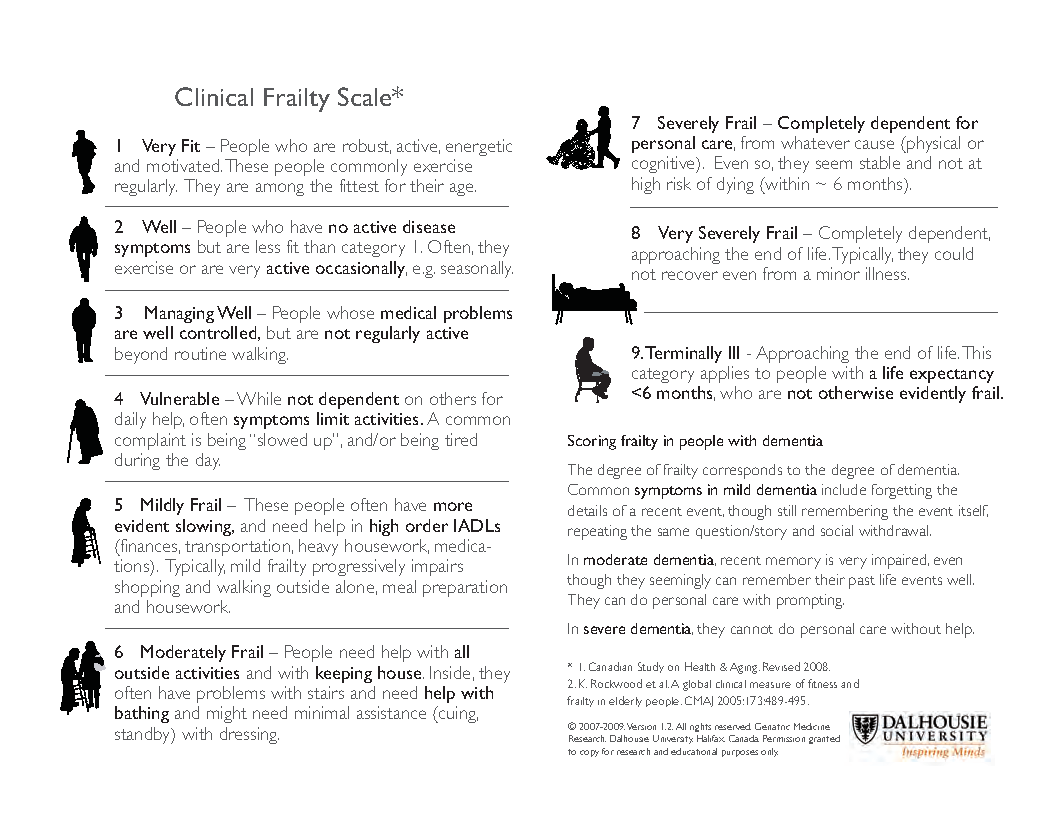
\includegraphics[width=\textwidth]{CFS}

%\end{appendix}

\end{document}
